In Year 1 we also performed simulations of the CHIMERA facility, developed by UKAEA, which enables validation of breeding blanket components under reactor-like thermal and magnetic conditions (Figure~\ref{fig:c456}). To support CHIMERA, we developed high-fidelity thermal-fluids models using separate all-hex meshes for solid and fluid regions, generated via \textit{tet-to-hex} conversion with prismatic boundary layers. Solid meshes include 60M elements; fluid meshes range up to 1.69B elements. Using the spectral element method at $N=9$, we resolve up to 1.1 trillion points—setting a record for thermal-fluids simulations in complex geometry. Overset grids manage solid-fluid interaction. Figure~\ref{fig:c456} shows turbulent velocity fields (left) and solid/fluid temperatures (right), providing key insights for fusion component optimization.

%%%%%%%%%%%%%%%%%%%%%%%%%%%%%%%%%%%%%%%%%%%%%%%%%%%%%%%%%%%%%%%%%%%%%%%%%%
\begin{figure}[htb!] \centering {\setlength{\unitlength}{1.0in}
\begin{picture}(6.500,1.730)(0,0.05)
\put(0.00,0.00){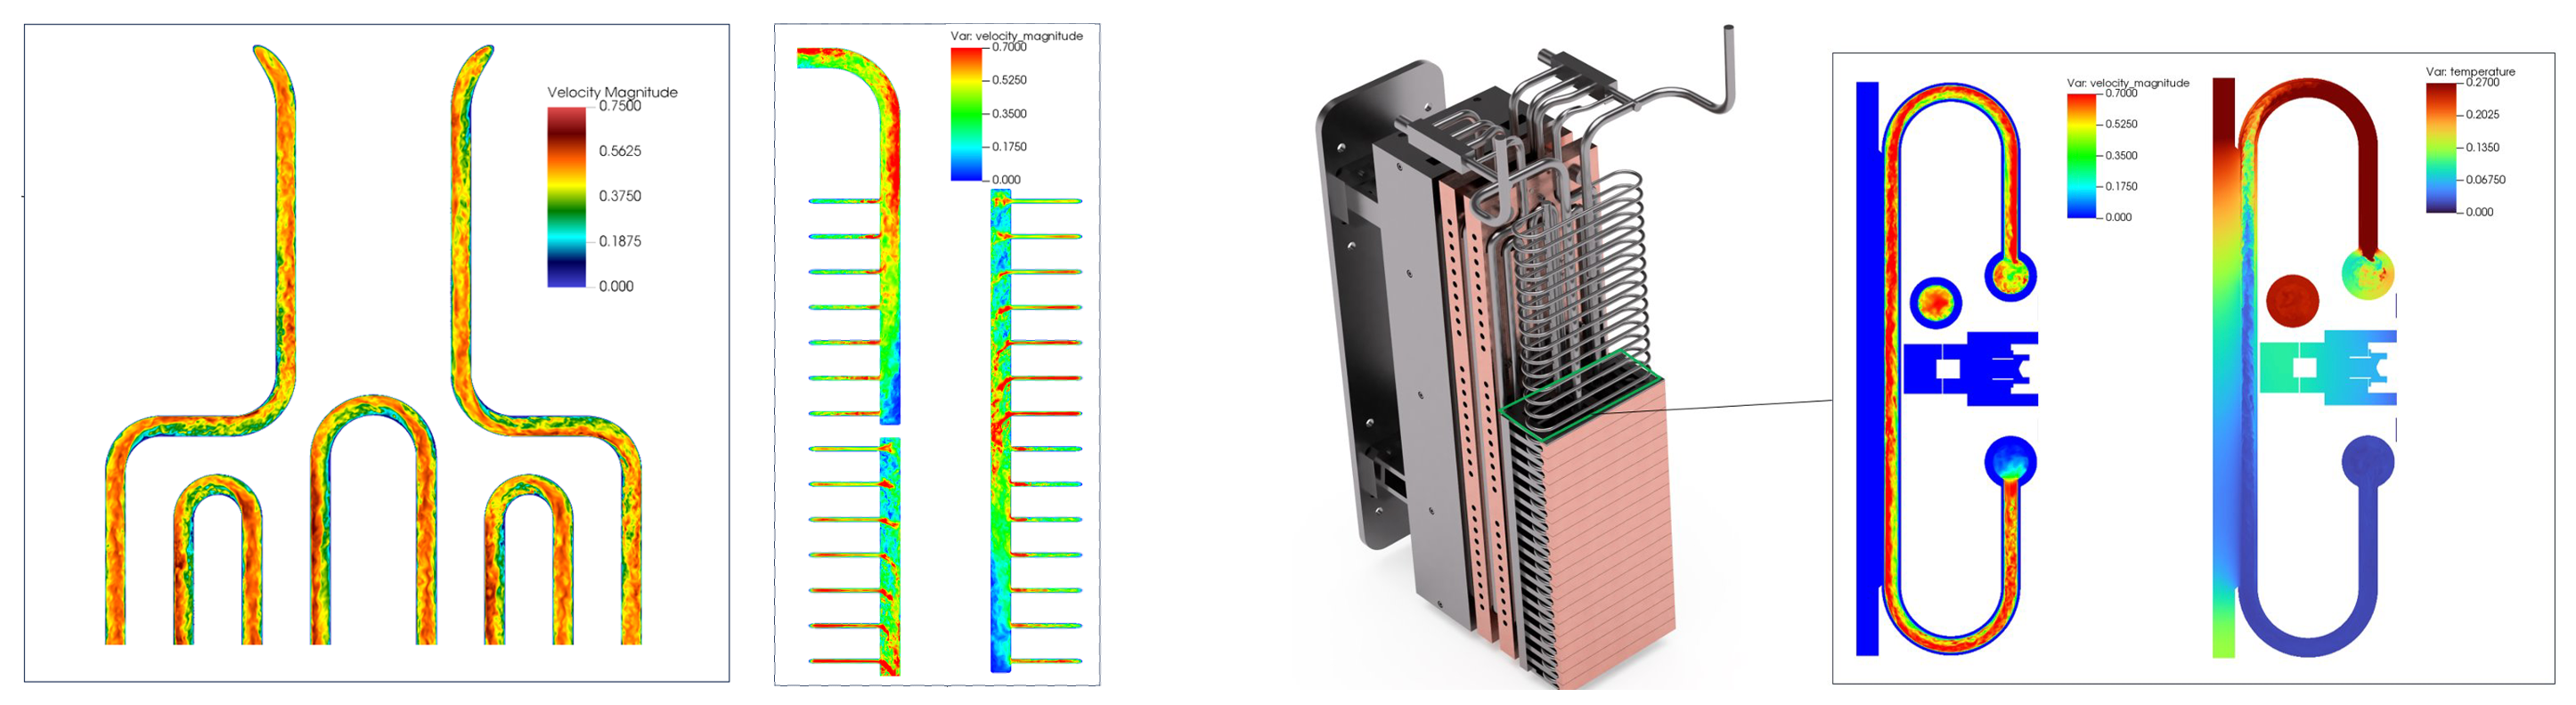
\includegraphics[width=6.50in]{figs/chimera_fluid2.png}}
\end{picture}}
\caption{\label{fig:c456}\small
CHIMERA results:
(left and left-center) instantaneous velocity magnitude in two cross-sections;
(right and right-center) solid and fluid temperatures.
}
\end{figure}
%%%%%%%%%%%%%%%%%%%%%%%%%%%%%%%%%%%%%%%%%%%%%%%%%%%%%%%%%%%%%%%%%%%%%%%%%%








